\chapter{Ievads}
%1.  Darba ievadā autors motivē temata izvēli, darba novitāti
ICT 2011. gada “ICT Facts Figure” statistisko datu apkopojums liecina, ka iedzīvotāju skaits ar platjoslas piekļuvi Internetam (ar pieslēgumu) ir pieaudzis par 45\% kopš 2006. gada un 2011 gadā sasniedza 5.9 miljardus mobilo Interneta lietotāju (\seename ~\figurename .~\ref{fig:mobilStat}, \cite{ict}). Rietumeiropas un Ziemeļamerikas reģionos mobilā interneta lietotāju skaits sasniedza 87\% no iedzīvotāju skaita. Tas nozīmē, ka 8 cilvēkiem no 10 bija pieejama mobilā ierīce, kas spēja nodrošināt bezvadu Interneta piekļuvi. To var izskaidrot sekojoši: Pirmkārt, ierīces cenas samazināšanās aptuveni no 2005.g. līdz 2006 g.; Otrkārt mobilā Interneta pieslēgumu cenas samazināšana ap 2007. gadu; un Treškārt liels lietojumprogrammu piedāvājuma klāsts kas izmanto Interneta piekļuvi. Mazas komunikāciju ierīces kļuva par neatņemamu sastāvdaļu daudzu lietotāju dzīvēs, un lietotāju vidū strauji izplatījās tādas ierīces kā - PDA, mobilie telefoni, multimediju atskaņotāji, spēļu konsoles un citas ierīces.
\begin{figure}[ht!]
    \centering
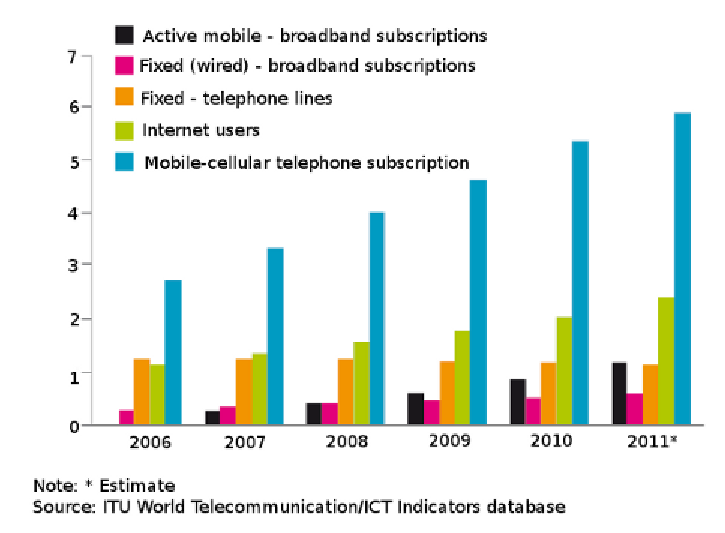
\includegraphics[scale=0.8]{./graph/mobuser1}
\caption{ICT lietotāju statistika laikā periodā 2006 - 2011 \cite{ict}}
\label{fig:mobilStat}
\end{figure}

Ekspromta tīklu plašais pielietojuma spektrs veicina gan šo tīklu ieviešanas pieaugošo intensitāti, gan arī nodrošina inovatīvo tehnoloģisko risinājumu pieaugumu. To, savukārt pastiprina aizvien pieaugošais lietojumprogrammu klāsts kuram sensoru tīkli ir paredzēti, sākot ar maza mēroga statiskiem tīkliem un līdz liela mēroga augsti mobiliem tīkliem. Pēdējā laikā ekspromta tīkli guva plašu interesi, un daudzi pētnieki saskata aiz vien pieaugošu potenciālu ekspromt tipa tīklu attīstībā. To pašreizējā attīstības stadija ir vēl tālu no tīkliem ar infrastruktūru. Un panākt Ad Hoc tīklā ātru, stabilu un uzticamu datu pārraidi ir grūts un ilgs process.
Taču, neraugoties uz to - jau šodien ar ekspromta tīklu palīdzību tiek izveidoti tīkli, kas ir paredzēti kādam vienam noteiktam mērķim, piemēram - tie tiek uzstādīti tādās vietās, kur infrastruktūras izveide nav iespējama \cite{self_manag}. Nākotnē, kad mobilo ekspromta tīklu pielietošana būs iespējama atbilstoši to pilnvērtīgam potenciālam, tiks nodrošināti tādi pakalpojuma veidi kas pieprasa stabilu savienojumu ar augstu \ac{QoS}, kā e-komercijas lietojumprogrammām, reāllaika video konferences, mobila režģa skaitļošanu (mobile grid computing), transportlīdzekļu sensora tīkls (\acs{VANET}) un daudzi citi.


%3. izvēlētās pētniecības metodes un objektus
\acf{QoS} prasības ir izstrādātas informācijas iegūšanai par lietotāja rīcībā esošajiem tehniskajiem resursiem, piemēram, datu apstrādes jaudas resursiem, datu uzglabāšanas resursiem un līdzīgi. Šādu prasību izstrādes nepieciešamību pamato ar plašo iekārtu daudzveidību un nepieciešamību nodrošināt to savstarpēju saderību un sadarbību. Kā rezultātā ir izstrādāti dažādu līmeņu QoS parametri un to izmantošanas kritēriji. Šie kritēriji var tikt tendēti uz jaudas parametru uzraudzību, attēlu rezolūcijas sinhronizācijas īpatnībām, dažādu platformu saderību, jeb pielagot citu parametru pielīdzināšanai kas būtiski ietekmē gan pārsūtāmo datu apjomu, gan, līdz ar to, arī kopējo QoS līmeni. Šī darba mērķis ir noteikt nepieciešamo BER līmeni kvalitatīvai datu pārraidei bezvadu sensor tīklos (WSN). Izmantojot diskrēto notiku datorsimulāciju un balstoties uz eksperimenta rezultātiem noteikt mobilitātes ietekmi uz QoS. Ņemot vērā laika ierobežojumu atvēlētu šī darba izstrādāšanai, pētīšanas apgabals tiks ierobežots sekojoši: a) tiks apskatīti plaši pielietojamo mobilitātes modeļu un komutācijas protokolu aspekti, b) tiks izvērtēta datu pārraides ātruma un maksimālo starpmezglu pārvietošanās ātrumu \gls{v_max} ietekme uz BER  un c) apskatīta dažādu protokolu veiktspēja mobilitātes apstākļos.
%4. un definē darba mērķus un uzdevumus,
Lai sasniegtu uzstādīto mērķi un skaitliskā viedā izteiktu mobilitātes ietekmi uz servisa kvalitāti (\acs{QoS}), šai darbā tiks veikts analītisks apskats par mobilajiem sensoru tīkliem un vēlāk darba gaitā tiks izstrādāta datorsimulācija \ac{NS-2} vidē. Lai sasniegtu mērķi ir nepieciešams:
\begin{enumerate}[label=\arabic*)]
\item Izpētīt mobilitātes ietekmi bezvadu sensoru tīklos (\acs{WSN}) un to ietekmi uz bitu kļūdu intensitāti (\acs{BER}).
\item Izpētīt mobilitātes ietekmi uz maršruta garuma daudzposmu maršrutā.
\item Balstoties uz eksperimentāli iegūtajiem rezultātiem (NS-2 simulācijas) izvērtēt analītiski iegūtos datus.
\end{enumerate}


\section{Literatūras apskats}\label{sec:lit}
Pēdējā laikā bezvadu sensoru tīkli (\acs{WSN}) piesaista lielu pasaules pētnieku interesi un tiek uzskatīti par potenciālu risinājumu visuresošai piekļuvei Internet tīklam \cite{perkinsBook,toh}. Šo vīziju īstenošana galvenokārt ir atkarīga no iespējas nodrošināt atbilstošu \acs{QoS} līmeni sensoru tīklos un tīkla mezglu mobilitāti. Nākamās paaudzes ekspromta tīkla (\acs{Ad Hoc}) mezgli būs mobili, piemēram, novietoti transportlīdzeklī \cite{dsdv_mobPc}. Izveidot un uzturēt daudzposmu savienojumu ir sarežģīts uzdevums nemitīgi mainošas topoloģijas apstākļos: daudzposmu maršrutā katra mezgla pozīcija nemitīgi mainās laikā un telpā. Tas rada nepieciešamību pārraudzīt visu mezglu novietošanu arī pēc maršruta izveidošanas, lai gadījumā, ja viens vai vairāki megli tiek izslēgti no aprites, tad vēl joprojām būtu iespējams uzturēt savienojumu starp gala punktiem \cite{park, lim, son}. R. Rao savā darbā \cite{rao} raksta, ka iepriekš projektēts mobilitātes modelis atstāj būtisku ietekmi uz eksperimenta rezultātiem.

2000. gadā P. Gupta un P.R. Kumar piedāvāja un pamatoja transportēšanas kapacitātes koncepciju \cite{gupta}. Koncepcija ņem vērā tīklā pārraidīto informācijas daudzumu un attālumu kādā šī informācija tiek pārraidīta. Šie parametri palīdz noteikt maksimāli ilgtspējīgu datu plūsmu daudzposmu ekspromta bezvadu tīklā. Tas nozīmē, ka teorētiski mobilitāte var paaugstināt tīkla datu pārraides kapacitāti (kā aprakstījis M.Grossglauser un D.Tse \cite{grossglauser}), bet praksē ekspromta tīkla (\acs{Ad Hoc}) tīkla veiktspēja samazinās mobilitātes dēļ \cite{perkins_hughes}. M.J.Neely un E.Modiano, lai sniegtu labāku priekšstatu par mobilitātes ietekmi pētāmais tīkls tiks apskatīts sadalīts šūnās, \seename \cite{neely1}. Tīkls ir vienības kvadrāts \footnote{kvadrāts Dekarta koordinātu sistēmā ar koordinātām (0, 0), (1, 0), (0, 1), un (1, 1)} kurā izvietoti mobilie mezgli. Šai gadījumā tīkls ir sadalīts šūnās, kas ir vienādas pēc izmēra un nepārklājas savā starpā, mezgli var izveidot savienojumu ja atrodas vienā un tajā pašā šūnā. Lai izvairītos no savstarpējiem mezglu traucējumiem (kā mezglu savstarpējie traucējumi  (\acs{INI})) tiek izmantotas četras dažādas frekvences (\seename ~\figurename .1, \cite{neely1}). Šis modelis balstīts uz kompromisu starp tīkla kapacitāti un pakešu aizkavi rindā. S.Toumpis savā darbā pēta maksimālo pārraides ātrumu un pārraides aizkaves augšējo robežu mobilajos mezglos sensora tīklā, ņemot vērā signāla rimšanas efektu \cite{toumpis}.

Jaunu paņēmienu ierosināja G.Ferrari un O.K.Tongus \cite{tonferBOOK}. Viņu ierosinātais paņēmiens atšķirās no \cite{neely1} aprakstītā un atšķirās ar to, ka statiski mezgli novietoti režģa četrstūros. Darbā tika izvērtēta tīkla veiktspējas izmaiņu atkarība no fiziskā slāņa īpašībām, kā arī analizēts vides piekļuves vadības (\acs{MAC}) protokols. Kombinējot rezervēšanas komutācijas (\acs{RBS}) metodi \cite{ferrari17} kā arī apskatot bez-rezervēšanas (\acs{NRBS}) metodi \cite{tonguz18}. Vēlāk savos darbos G.Ferrari un O.K.Tongus pēta mezglu mobilitātes ietekmi uz BER līmeni izmantojot to pašu mezglu izvietojumu \cite{tonferBOOK}.

Pārsvarā zinātniski raksti, kas ir publicēti par tēmu „Mobilie ekspromta tīkli”, savu pētījumu eksperimentālajā daļā izmanto IEEE 802.11 protokolu. IEEE 802.11 protokolā datu pārraidei tiek izmantots Wi-Fi vai Bluetooth interfeiss. Nesen tika izveidots jauns iterfeisa standarts - IEEE 802.15.4/ZigBee, kas vēl nav tik "populārs" kā IEEE 802.11.

\section{Tēmas aktualitātes pamatojums}
Kā jau iepriekš apskatīts, tad ekspromta tīklu pielietojums ikdienā kļūst aizvien plašāk izplatīts un ieņem aizvien būtiskāku lomu ikdienas vajadzību nodrošināšanā. Kā vienu no šāda mērķa sasniegšanas risinājumiem var uzskatīt vienu no jaunākajiem izstrādātajiem un IEEE apstiprinātajiem standartiem - 802.15.4/ZigBee. Šis protokols ir izstrādāts ar mērķi uzlabot un nodrošināt sensoru un kontroles pielietojamības iespējas mobilajos tīklos. Standarts paredz dažāda veida tīkla pašatjaunošanās iespējas. Tas, savukārt, nodrošina efektīvākus tīklu savstarpējās saslēgšanas risinājumus ar samazinātu enerģijas jaudu, kas savukārt palielina mobilo iekārtu mobilitāti un pagarina to darbības laiku.

Zinātniskajos institūtos visā pasaulē aiz vien lielāka uzmanība tiek pievērsta dzīves kvalitātes uzlabošanai, kas savukārt rada nepieciešamību organizēti grupēt un savstarpēji savienot plašu klāstu ekspromta tīklu. Kā piemēru var minēt Oslo inovāciju centra izstrādes stadijā esošo veselības aprūpes komplekso risinājumu - Dignio \cite{dingio}.
Dignio projekts paredz ražošanā ieviest kompleksu iekārtu, kuras uzdevums ir nodrošināt savienojumu ar plašu klāstu mobilo iekārtu risinājumiem, kā WLAN, WPAN, ZigBee, NFC un daudzi citi. Šādi risinājumi ne tikai būtiski veicina mobilā interneta piekļuves iespējas, taču vienlaicīgi nodrošina augsto tehnoloģiju un risinājumu ieviešanu ikdienas dzīvē, nodrošinot lietotājiem ne tikai divpusēju savienojumu ar uzraudzības centrāli, taču arī savienojumu ar vairumu ikdienā lietojamo bezvadu iekārtu. Šādu risinājumu izstrāde ir komplicēts darbs un prasa lielus resursu ieguldījumus zinātniskajā darbā.

Lai attiecīgajos risinājumos nodrošinātu augsta līmeņa iekārtu komunikāciju kvalitāti ir būtiski izvērtēt nepieciešamību nodrošināt lietotājam vienu no būtiskākajām prasībām - mobilitāti. Kas savukārt rada palielinātas prasības QoS nodrošināšanai jo pieaugot lietotāju mobilitātei tīklā var parādīties stohastiski raksturlielumi kas var būtiski ietekmēt QoS. Tādējādi šī maģistra darba tēmas aktualitāti var skaidrot ar nepieciešamību nodrošināt lietotājiem mobilitātes iespējas neatkarīgi no to prasībām.

\section{Pētāma tīkla parametri }\label{sec:petPar}
Mobilais sensoru tīkls tiek pieņemts ar sekojošiem parametriem:
\begin{enumerate}
	\item Datu pārraidei tiek izmantota $f_{c} = 915$ [MHz] frekvence.
 	\item Tīklam ir kvadrāta forma ar laukumu $S = 1500\times300$ un $500\times300$, [$m^{2}$]. Tīkla laukums ir konstants un nemainīgs simulācijas laikā.
  	\item Tīkla laukumā $S$ viendabīgi izkliedēti $N$ mobilie mezgli. Reālajā dzīvē tas varētu izpausties kā fakultātes vai lidostas ēka ar laukumu $S$, kurā pārvietojas cilvēki ar portatīviem datoriem vai/un mobiliem telefoniem. Cilvēki pārvietojas ēkā neaizejot ārpus tā laukuma, tajā pašā laikā cilvēku blīvums ēkā ir mainīgs $\rho_{s} = \frac{N}{S}$.  Mezglu skaits ir konstants lielums un $N = 51$ mezgls.
  	\item Katra mezgla pārraides jauda ir konstants lielums \gls{p_t} $= 1$ [mW] un tā minimālā uztveres jauda \gls{p_imin} $= - 94$ [dBm] arī konstants lielums.
  	\item Trafika ģenerēšanai tiek izmantots konstants bitu ātrums (\acs{CBR}) ar paketes garumu \gls{L} $= 512$ [b/pck] un datu pārsūtīšanas ātrums \gls{r_b} $= 2$ [Mbit/s]. CBR tiek izvēlēts, lai izslēgtu varbūtību, kā trafika variācija var ietiekmēt eksperementu rezultātus, līdz ar to labākais variants ir izvēlēties konstants trafiks. 
  	\item Starpmezglu interference. No vienādojuma (\ref{eq:ini}) izriet - lai samazinātu starpmezglu interferences līmeni ir nepieciešams lai $\lambda L/R_{b}$ būtu pēc iespējas mazs lielums (\seename~\cite{qoS_static}). Tiek uzskatīts, ka avota ražo informāciju  paketes. Katrs mezgls izveido paketes konstantā garumā pēc Puassona sadalījuma ar \gls{lambda} = 4 [pck/s].
  	\item Kanāla modulācija ir  binārā fāzes manipulācija (\acs{BPSK}).
  	\item Maršruta izveidošanas stadija netiek apskatīta un netiek ņemta vēra simulācijas rezultātu analīzē. Kā minēts \ref{sec:prot} nodaļā maršruta izveidošana ir viens no svarīgiem un sarežģītiem procesiem sensoru tīklā \cite{perkinsBook}. Lai sasniegtu šī darba uzstādīto mērķi (datu apmaiņas procesa pētīšana) tīkls tiks pētīts pēc sākotnēja maršrutu izveidošanas procesa.
  	\item Izmantots gadījuma maršrutpunktu mobilitātes modelis (\acs{RWMM}).
  	\item Starpmezgls ziņojumu nepārraida tālāk kamēr nav saņēmis visu ziņojumu.
  	\item Tiek pieņemts, ka komunikāciju kanāls ir ideāls: kaimiņ-mezgls uz $r_{link}$ distances ir nekavējoties pieejams.
	\item Enerģijas patēriņš netiks ņemts vērā darba gaitā.
\end{enumerate}

\section{Darba pārskats}
%5. sniedz nelielu ieskatu katrā no darba nodaļām numeroloģiskā secībā.
Šis darbs ir organizēts pēc sekojoša principa: Nodaļā \ref{sec:infra} apskatīti ekspromta tīklu veidi. Nodaļā \ref{sec:tris} ir apkopoti Ad hoc tīklu teorētiskie aspekti, kā tīkla formas matemātiskie interpretācijas veidi, BER aprēķināšanas veidi, mezglu ātrums un komutācijas veidi: Bez-rezervēšanas (\acs{NRBS}) un rezervēšanas-bāzētas (\acs{RBS}). Nodaļā \ref{sec:mobilityModels} ir apskatīti trīs visplašāk pielietojamie mobilitātes modeļi mobilo Ad hoc tīklu simulācijas: \acf{RWMM},\acf{RDMM} un \acf{OMM}. Kā arī \acs{RWMM} modelim ir aprakstīta daudzposmu maršruta garuma izmaiņa mobilitātes ietekmē. Nodaļā \ref{sec:prot} ir sniegts neliels ekspromta tīklu maršrutēšanas protokolu apskats tādiem protokoliem kā: \acf{AODV}, \acf{DSR} un \acf{OLSR}, kā arī piedāvāts jauns maršrutēšanas algoritms SP-BER.  Daži no šiem protokoliem ir vēlāk izmantoti NS-2 simulāciju scenārijos. Nodaļā \ref{sec:prakt} aprakstīti NS-2 simulācijas scenāriji un to rezultāti. Nobeiguma nodaļā \ref{sec:secin} ir izklāstīti secinājumi.